% !TEX program = xelatex
\documentclass[10pt,letterpaper,twocolumn]{article}

\usepackage[top=0.75in, bottom=0.75in, left=0.75in, right=0.75in]{geometry}
\usepackage{fontspec}
\usepackage{unicode-math}
\setmainfont{Latin Modern Roman}[
  Extension=.otf,
  UprightFont=lmroman10-regular,
  BoldFont=lmroman10-bold,
  ItalicFont=lmroman10-italic,
  BoldItalicFont=lmroman10-bolditalic,
]
\setsansfont{Latin Modern Sans}[
  Extension=.otf,
  UprightFont=lmsans10-regular,
  BoldFont=lmsans10-bold,
  ItalicFont=lmsans10-oblique,
  BoldItalicFont=lmsans10-boldoblique,
]
\newfontfamily\acbold{ywft-processing-bold}[Path=../../system/public/type/webfonts/,Extension=.ttf]
\setmonofont{Latin Modern Mono}[
  Extension=.otf,
  UprightFont=lmmono10-regular,
  ItalicFont=lmmono10-italic,
  Scale=0.85,
]

\usepackage{xcolor}
\usepackage{titlesec}
\usepackage{enumitem}
\usepackage{booktabs}
\usepackage{tabularx}
\usepackage{fancyhdr}
\usepackage{hyperref}
\usepackage{xurl}
\usepackage{graphicx}
\graphicspath{{figures/}{../arxiv-ac/figures/}}
\usepackage{ragged2e}
\usepackage{microtype}
\usepackage{natbib}
\usepackage{tikz}
\usetikzlibrary{positioning,arrows.meta,fit}
\usepackage{pgfplots}
\pgfplotsset{compat=1.18}
\usepackage{../ac-source-bundle}
\usepackage{balance}

\definecolor{acpink}{RGB}{180,72,135}
\definecolor{acpurple}{RGB}{120,80,180}
\definecolor{acdark}{RGB}{64,56,74}
\definecolor{acgray}{RGB}{119,119,119}
\definecolor{aclight}{RGB}{226,214,236}

\hypersetup{colorlinks=true,linkcolor=acpurple,urlcolor=acpurple,citecolor=acpurple,
  pdftitle={What People Type at the Prompt},
  pdfauthor={@jeffrey}}

\titleformat{\section}{\normalfont\bfseries\normalsize\uppercase}{\thesection.}{0.5em}{}
\titlespacing{\section}{0pt}{1.2em}{0.3em}
\titleformat{\subsection}{\normalfont\bfseries\small}{\thesubsection}{0.5em}{}
\titlespacing{\subsection}{0pt}{0.8em}{0.2em}

\newcommand{\acdot}{{\color{acpink}.}}
\newcommand{\ac}{Aesthetic{\acdot}Computer}

\pagestyle{fancy}\fancyhf{}
\renewcommand{\headrulewidth}{0pt}
\fancyhead[C]{\footnotesize\color{acpink}\textit{Field report --- \ac{} papers}}
\fancyfoot[C]{\footnotesize\thepage}

\newcommand{\code}[1]{\texttt{#1}}
\renewcommand{\dbltopfraction}{0.8}
\setcounter{dbltopnumber}{2}

\setlist[itemize]{nosep, leftmargin=1.2em, itemsep=0.1em}
\setlist[enumerate]{nosep, leftmargin=1.4em, itemsep=0.1em}
\setlength{\columnsep}{1.8em}
\setlength{\parindent}{1em}
\setlength{\parskip}{0.3em}

\tolerance=800
\emergencystretch=1em
\hyphenpenalty=50

\begin{document}

\twocolumn[{%
\begin{center}

\includegraphics[height=4em]{pals}\par\vspace{0.5em}
{\acbold\fontsize{21pt}{25pt}\selectfont\color{acdark} What People Type at the Prompt}\par
\vspace{0.45em}
{\normalfont\itshape\fontsize{11pt}{13pt}\selectfont\color{acpink} Fifty-four days of the \ac{} prompt log, and a live count of who is here}\par
\vspace{0.3em}
{\normalfont\fontsize{9pt}{11pt}\selectfont\color{acgray} 5,273 entries, one clock that takes most of them, and how few of the misses are really misses.}\par
\vspace{0.6em}
{\normalsize\href{https://prompt.ac/@jeffrey}{@jeffrey}}\par
{\small\color{acgray} \ac{} --- October 26, 2026}\par
{\small\color{acgray} ORCID: \href{https://orcid.org/0009-0007-4460-4913}{0009-0007-4460-4913}}\par
\vspace{0.3em}
{\small\color{acpurple} \url{https://aesthetic.computer}}\par
\vspace{0.6em}
\rule{\textwidth}{1.5pt}
\vspace{0.5em}
\end{center}

\begin{quote}
\small\noindent\textbf{Abstract.}
The prompt is the front door of \ac{}: a visitor types a word and lands in a
piece. Since 3~September 2026 every submission has been recorded anonymously,
with the text, a coarse kind, whether it resolved, and an hour-rounded time.
This report reads the whole log through 26~October: 5,273 entries over
54~days, 2,431 of them in the last 30 and 590 in the last seven. One piece,
the Danish chat clock \code{laer-klokken}, accounts for 57\% of all entries.
The logger marks 725 entries (14\%) as unresolved, but 28\% of those are
commands the prompt answers itself and another 28\% are misspellings of pieces
that exist, 96 of them of \code{laer-klokken} alone. Genuine misses are 6\% of
traffic. Daily volume has a median of 84, one spike of 652 on 19~September,
and a decline of about a fifth from the first half to the second once that
spike is set aside. We also describe the live counterpart shipped alongside
this report, a session-server endpoint and piece that show which handles and
how many guests are on \ac{} now, and two defects it exposed.
\end{quote}
\vspace{1em}
}]

\section{Introduction}
\label{sec:intro}

\ac{} is used by typing. A visitor types \code{notepat} and gets an
instrument, \code{chat} and gets a room, a dollar code and gets a KidLisp
program \citep{scudder2026ac,scudder2026kidlisp}. The prompt is therefore the
most direct record of intent the system has: not what a page offered, but what
someone asked for. When the word names nothing, the prompt says so, and the
visitor tries again or leaves.

Until September that record was thrown away. A small logger now keeps it, and
after seven weeks there is enough to ask three questions. What do people type?
How often does the prompt fail them, and why? And what does the shape of the
traffic say about who is using \ac{} right now? The last question has a live
form too, which we answer with a separate, stateless view of presence
(Section~\ref{sec:presence}).

\section{Context}
\label{sec:context}

Earlier audits counted the network from the outside --- handles, published
pieces, paintings and moods --- and asked who uses \ac{} and what they make
\citep{scudder2026network}. Those are records of things finished. The prompt
log records things attempted, including the attempts that failed, which is the
part a product usually never sees. Addressing by name is a deliberate
choice: pieces are URL-addressable words, and the system bets that a short
vocabulary can be memorized like fingerings on an instrument
\citep{scudder2026url}. A failed word is a measure of where that bet does not
hold, in the sense that a door with the wrong handle is a design failure and
not a user's \citep{norman1988design}.

\section{System}
\label{sec:system}

\subsection{The prompt log}

When a visitor submits text, the prompt piece posts it, fire-and-forget, to
\code{/api/prompt-log} \citep{acrepo2026}. The handler stores five fields: the
text (trimmed, at most 256 characters), a \emph{kind}, a \emph{resolved}
flag, the UTC day, and a timestamp rounded down to the hour so that rows
cannot be strung into one person's sequence. It stores no handle, account or
address. The client address is used only as a key in an in-memory,
one-minute rate limiter and is never written. Arguments to \code{email} are
replaced with \code{[redacted]}.

Kind is decided by a short rule. Text that opens with a parenthesis or
contains a newline is \emph{kidlisp-source}. A dollar code is
\emph{kidlisp-code}, resolved if the code exists. Text beginning with
\code{@} is a \emph{user-piece}, unresolved by design. Otherwise the first
word, cut at any colon or tilde, is looked up as a piece on disk; a hit is a
\emph{piece}, and anything else is a \emph{word} with \code{resolved=false}.
That last bucket is what the logger treats as the miss corpus.

\subsection{Live presence}
\label{sec:presence}

The log answers \emph{what}, after the fact. \emph{Who is here now} lives in
the session server, which holds one socket per open \ac{} tab. Signed-in tabs
report their handle and, on each piece change and every 2.5~s as a
keep-alive, their current piece. We added a public \code{/visitors} endpoint
that returns handles with their current piece and tab count, and a bare guest
count, deduplicated by address and never returning one. A \code{visitors}
piece polls it every five seconds and runs fullscreen on a wall display
(Figure~\ref{fig:flow}).

\begin{figure}[t]
\centering
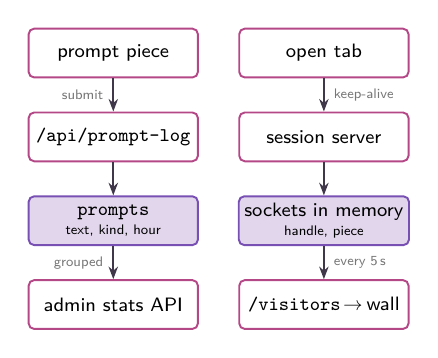
\begin{tikzpicture}[
  node distance=0.42cm and 0.5cm,
  box/.style={draw=acpink, line width=0.7pt, rounded corners=2pt, font=\sffamily\scriptsize, align=center, minimum width=2.15cm, minimum height=0.62cm, inner sep=2pt},
  store/.style={box, draw=acpurple, fill=aclight},
  arr/.style={-{Stealth[length=1.6mm]}, line width=0.6pt, color=acdark},
  lab/.style={font=\sffamily\tiny, color=acgray}
]
\node[box] (prompt) {prompt piece};
\node[box, below=of prompt] (log) {\code{/api/prompt-log}};
\node[store, below=of log] (db) {\code{prompts}\\[-1pt]{\tiny text, kind, hour}};
\node[box, below=of db] (stats) {admin stats API};

\node[box, right=of prompt] (tab) {open tab};
\node[box, below=of tab] (ss) {session server};
\node[store, below=of ss] (mem) {sockets in memory\\[-1pt]{\tiny handle, piece}};
\node[box, below=of mem] (vis) {\code{/visitors}\,$\rightarrow$\,wall};

\draw[arr] (prompt) -- node[lab, left] {submit} (log);
\draw[arr] (log) -- (db);
\draw[arr] (db) -- node[lab, left] {grouped} (stats);
\draw[arr] (tab) -- node[lab, right] {keep-alive} (ss);
\draw[arr] (ss) -- (mem);
\draw[arr] (mem) -- node[lab, right] {every 5\,s} (vis);
\end{tikzpicture}
\caption{The two records. Left: the prompt log keeps what was typed, without
identity, indefinitely. Right: presence keeps who is connected, only while they
are, and is never written down.}
\label{fig:flow}
\end{figure}

\subsection{Two defects the presence work exposed}

Building the endpoint turned up two faults in the session server, both fixed
in the same commit. First, a security change that morning had moved the
server behind a local proxy, so every socket arrived from \code{127.0.0.1}
and all guests collapsed into one. The server now reads the forwarded address,
and only when the hop is loopback. Second, the message dispatcher matched
\code{location:broadcast} twice, and the first branch was an empty,
commented-out body. Every location message fell into it, so no visitor's
current piece had been recorded, and the profile presence that depends on it
had been silent. Removing the dead branch restored both. The public status
page, which listed raw addresses, no longer does.

\section{Method}
\label{sec:method}

We took one snapshot through the admin stats API at 04:20~UTC on
27~October. The API groups identical texts and returns kind totals, each
group's first and last appearance, and at most 500 groups. Three windows were
read: all time (from 3~September), 30~days (from 27~September) and seven days
(from 20~October). The 500 most frequent texts cover 92.9\% of all-time
entries and every entry in the two shorter windows. A daily series, which the
API does not offer, was rebuilt by asking for the count from each UTC day
onward and differencing consecutive days. It sums to 5,256 through
26~October; the remaining 17 entries fall on the first hours of the 27th.

Unresolved entries were sorted into six classes. \emph{Internal} entries begin
with one of the 136 commands that \code{prompt.mjs} handles itself
(\code{signup}, \code{login}, \code{done}, \code{channel}, \code{resize}
and so on), which the logger cannot see. \emph{Clock spellings} match a
pattern for \code{laer-klokken} written without its hyphen, with
\emph{\ae}, truncated or transposed. \emph{Near-misses} differ from a piece
name only in case or punctuation, or lie within edit distance two
\citep{levenshtein1966binary} for words of six letters or more, one for five.
Shorter words are never counted as typos, because at that length almost every
English word is one edit from some piece. \emph{Sentences} have three words or
more, \emph{codes} begin with \code{\#} or \code{\$}, and the rest are
\emph{words}. Aggregate tables and the series are in \code{data/}; the raw
snapshot is not published (Section~\ref{sec:ethics}).

\section{Results}
\label{sec:results}

\subsection{Volume}

\begin{figure*}[t]
\centering
\begin{tikzpicture}
\begin{axis}[
  width=\textwidth, height=4.6cm,
  ybar=0pt, bar width=5.2pt,
  ymin=0, ymax=200, xmin=-1, xmax=54,
  axis lines*=left, axis line style={acgray},
  tick style={acgray}, tick label style={font=\sffamily\scriptsize, color=acdark},
  ylabel={entries per day}, ylabel style={font=\sffamily\scriptsize, color=acdark},
  xtick={0,7,14,21,28,35,42,49}, xticklabels={Sep 3,Sep 10,Sep 17,Sep 24,Oct 1,Oct 8,Oct 15,Oct 22},
  ytick={0,50,100,150,200},
  ymajorgrids, grid style={aclight},
  legend style={font=\sffamily\scriptsize, draw=none, fill=none, at={(0.99,0.97)}, anchor=north east, legend columns=2},
  legend image code/.code={\draw[#1, draw=none] (0cm,-0.08cm) rectangle (0.28cm,0.14cm);},
  clip=false,
]
\addplot[fill=acpink!55, draw=none, bar shift=0pt] table[x expr=\coordindex, y expr={min(\thisrow{total},200)}, col sep=comma] {data/daily.csv};
\addplot[fill=acpurple, draw=none, bar shift=0pt] table[x expr=\coordindex, y expr={min(\thisrow{unresolved},200)}, col sep=comma] {data/daily.csv};
\legend{all entries, logged as unresolved}
\draw[acdark, line width=0.5pt] (axis cs:16,203) -- (axis cs:16,214);
\node[font=\sffamily\scriptsize, color=acdark, anchor=west] at (axis cs:16.4,214) {Sep 19: 652 entries (180 unresolved), bar cut at 200};
\end{axis}
\end{tikzpicture}
\caption{Prompt entries per UTC day, 3~September to 26~October 2026. The
first day is partial. The 19~September bar is cut at 200 to keep the other
53 days readable.}
\label{fig:daily}
\end{figure*}

Over 54 days the prompt took a mean of 97 entries a day and a median of 84
(Figure~\ref{fig:daily}). One day dominates the mean: on 19~September there
were 652 entries, 180 of them unresolved, and 136 entries that day were texts
seen on no other day --- requests for \code{snakes} and \code{notepad},
Danish greetings, misspellings of the clock. The log alone cannot say who they
were; the date coincides with a scheduled workshop, and the mix of languages
suggests more than one room. Setting that day aside, the first 27~days
averaged 96 entries and the last 27 averaged 78, a decline of about 19\%.

\begin{table}[t]
\centering
\small
\begin{tabular}{@{}lrrr@{}}
\toprule
kind & all time & 30 days & 7 days\\
\midrule
piece & 4,444 & 2,090 & 491\\
word (unresolved) & 724 & 278 & 89\\
kidlisp-source & 68 & 49 & 4\\
user-piece & 19 & 8 & 2\\
kidlisp-code & 18 & 6 & 4\\
\midrule
total & 5,273 & 2,431 & 590\\
\bottomrule
\end{tabular}
\caption{Entries by kind for the three windows, as the logger classifies them.}
\label{tab:kinds}
\end{table}

Most traffic opens a piece (Table~\ref{tab:kinds}): 84\% all time, 86\% over
30 days, 83\% over seven. KidLisp arrives mostly as pasted source rather than
as dollar codes, and user pieces addressed by \code{@handle} are rare.

\subsection{What people open}

\begin{table}[t]
\centering
\small
\begin{tabular}{@{}lr@{\hspace{1.4em}}lr@{}}
\toprule
\multicolumn{2}{@{}l}{all time} & \multicolumn{2}{l@{}}{30 days}\\
\midrule
\code{laer-klokken} & 2,984 & \code{laer-klokken} & 1,462\\
\code{laklok} & 188 & \code{laklok} & 91\\
\code{list} & 141 & \code{camera} & 48\\
\code{chat} & 101 & \code{list} & 44\\
\code{camera} & 82 & \code{chat} & 39\\
\code{notepat} & 58 & \code{handle} & 19\\
\code{song} & 50 & \code{notepat} & 18\\
\code{handle} & 43 & \code{mood} & 13\\
\code{pruttivox} & 42 & \code{pruttivox} & 13\\
\code{girlfriend} & 38 & \code{baktok} & 12\\
\code{help} & 24 & \code{valbear} & 12\\
\code{baktok} & 22 & \code{help} & 12\\
\bottomrule
\end{tabular}
\caption{Most-opened pieces, grouping every entry by its first word (so
\code{line:4 red} counts as \code{line}).}
\label{tab:pieces}
\end{table}

One piece takes most of the traffic (Table~\ref{tab:pieces}).
\code{laer-klokken}, a Danish chat clock, is 57\% of every entry ever logged,
60\% over 30~days and 45\% over the last week; its English-named sibling
\code{laklok} is second. Behind them the list is short and social:
\code{list} and \code{help} for finding things, \code{chat}, \code{handle}
and \code{mood} for presence, \code{camera}, \code{notepat} and \code{song}
for making. At least 140 distinct pieces were opened all time, 139 in the last
30 days and 85 in the last week.

\subsection{What fails, and why}

\begin{table}[t]
\centering
\small
\begin{tabular}{@{}lrrr@{}}
\toprule
class & all time & 30 days & 7 days\\
\midrule
internal command & 204 & 104 & 24\\
clock spelling & 96 & 21 & 7\\
near-miss of a piece & 107 & 37 & 18\\
word & 290 & 108 & 39\\
sentence & 23 & 5 & 1\\
code & 5 & 3 & 0\\
\midrule
logged unresolved & 725 & 278 & 89\\
genuine misses & 318 & 116 & 40\\
\quad share of all entries & 6.0\% & 4.8\% & 6.8\%\\
\bottomrule
\end{tabular}
\caption{Unresolved entries reclassified. Genuine misses are words,
sentences and codes; the first three rows are entries the system could have
answered.}
\label{tab:misses}
\end{table}

The logger's miss rate overstates failure by more than half
(Table~\ref{tab:misses}). Of 725 unresolved entries, 204 are commands the
prompt handled correctly but the logger cannot recognize --- \code{done},
\code{signup}, \code{login}, \code{channel}. Another 203 name a piece that
exists: 96 are the clock without its hyphen, with \emph{\ae}, cut short or
transposed (\code{laer}, \code{lær klokken}, \code{laerklokken},
\code{laer-klokke}), and 107 are near-misses of other pieces, led by
\code{notepad} for \code{notepat} and \code{radio} for \code{r8dio}. What
remains --- 318 entries, 6\% of traffic --- are genuine misses. They are
mostly single words that read as wishes: \code{snake}, \code{hello},
\code{music}, \code{circle}, \code{dog}, \code{cat}, colours. Sentences are
few, and are mostly greetings or messages addressed to a person, typed where a
chat box was expected.

\section{Discussion}
\label{sec:discussion}

\textbf{The clock is the audience.} More than half of all prompt traffic is
one community returning to one room, many times a day. Averages over the whole
log describe that community first and everyone else second, and any change to
\code{laer-klokken} moves every number here.

\textbf{The cheapest fix is aliases.} The clock's name is hard to type on an
English keyboard and harder from memory, and it fails 96 times in the log.
Routing \code{laer}, \code{lær}, \code{laerklokken} and close variants to the
piece, and \code{notepad} to \code{notepat}, would recover most of the
near-miss class with no new pieces.

\textbf{Fix the instrument before reading it.} The miss metric should learn
the prompt's own command list, so that \code{signup} stops counting as
failure. Until it does, the logger's raw rate is the wrong number to watch.

\textbf{Wishes are a backlog.} The genuine misses are a short list of things
people expected to exist. \code{hello} recurs from the first week to the
last, \code{snake} for a month after the spike; a \code{hello} that answers back may be worth more than another
piece nobody asks for.

\section{Ethics, privacy and limitations}
\label{sec:ethics}

\textbf{What is kept.} The log is anonymous by construction, but it keeps free
text indefinitely, and some of that text is personal: names, greetings,
messages meant for someone else. This report quotes only command words and
piece names and summarizes sentences by category. The raw snapshot stays with
the author. A retention limit on raw text, keeping only aggregates past a set
age, would match how the data is used.

\textbf{Entries are not people.} One visitor retrying ten times is ten
entries, and nothing in the log can say how many people the 5,273 entries
represent. Hour-rounding prevents reconstructing sessions, by design.

\textbf{Method limits.} Days are UTC, which splits a Copenhagen or Los Angeles
evening. The all-time piece table rests on the top 500 texts (92.9\% of
entries). The miss classes are heuristics; the near-miss rule is deliberately
strict and undercounts typos of short names. The presence view counts guests
by address, so a shared connection is one guest, and the display showing it
counts itself.

\section{Conclusion}
\label{sec:conclusion}

The prompt mostly works. Five in six entries open a piece, and of the rest
more than half were answered or nearly answered. Real failure is about one
entry in sixteen, concentrated in a handful of wishes and one hard name. The
log is small and new, and its main lesson so far is about the log itself: it
must know what the prompt knows before its misses mean anything. Presence,
now visible and fixed, is the other half --- the log says what people looked
for, the wall says who is here looking.

\balance
\bibliographystyle{plainnat}
\bibliography{references}

\end{document}
